\documentclass[12pt,letterpaper]{beamer}
\usetheme{Copenhagen}
\usecolortheme{seahorse}
\setbeamertemplate{section in toc}{\inserttocsection}

\usepackage[utf8]{inputenc}
\usepackage{amsmath}
\usepackage{amsfonts}
\usepackage{amssymb}
\usepackage{graphicx}
\graphicspath{ {./images/} }
\usepackage{hyperref}
\hypersetup{
    colorlinks=true,
    linkcolor=blue,
    filecolor=magenta,      
    urlcolor=cyan,
    pdftitle={Overleaf Example},
    pdfpagemode=FullScreen,
}
\title[Robotics I]
{ENGR 3421: ROBOTICS I}
\subtitle{Into the Autonomous Ground Vehicle}

\author[Zhang, Lin]
{Dr. Lin Zhang}
\institute[UCA] % (optional)
{
  Department of Physics and Astronomy\\
  University of Central Arkansas
}
\date[Robotics1 2021] % (optional)
{August 24, 2021}
\logo{
\includegraphics[height=1cm]{uca_bear_logo.png}}


%End of title page configuration block
%------------------------------------------------------------

%------------------------------------------------------------
%The next block of commands puts the table of contents at the beginning of each section and highlights the current section:

\AtBeginSection[]
{
  \begin{frame}
    \frametitle{Outline}
    \tableofcontents[currentsection]
  \end{frame}
}
%------------------------------------------------------------

\begin{document}

%The next statement creates the title page.
\frame{\titlepage}

%---------------------------------------------------------
%This block of code is for the table of contents after the title page
\begin{frame}
\frametitle{Outline}
\tableofcontents
\end{frame}
%---------------------------------------------------------


\section{Review}

\begin{frame}{Safety}
    \begin{alertblock}{Safe First!}
        Don't forget eyes and hands protection!
    \end{alertblock}
    We have gloves and first aid kit now.
\end{frame}

\begin{frame}{Version Control}
    \begin{itemize}
        \item Github provides hosting service.
        \item \href{https://git-scm.com/about}{Git} controls versions.   
    \end{itemize}        
    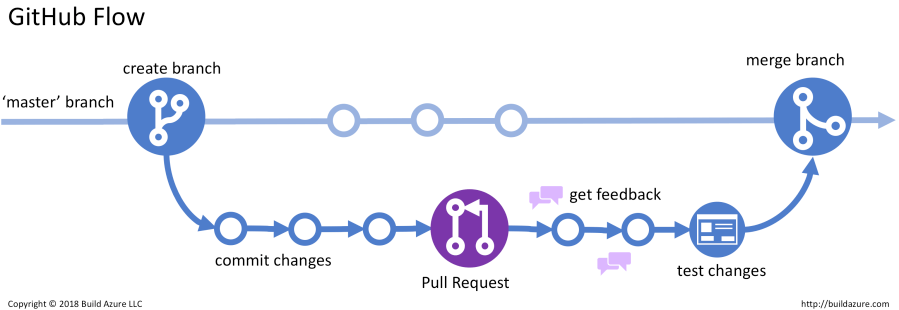
\includegraphics[width=.65\textwidth]{git_flow}
    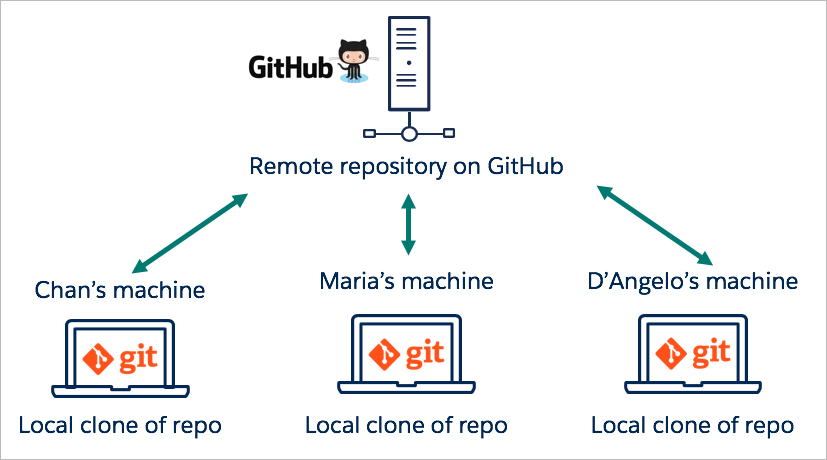
\includegraphics[width=.3\textwidth]{github_and_clones}
\end{frame}

\begin{frame}{Version Control}
    \begin{itemize}
        \item Getting started \href{https://docs.github.com/en/get-started}{guides} and \href{https://guides.github.com/activities/hello-world/}{Hello World}. 
        \item Alternatives: 
        \begin{itemize}
            \item \href{https://about.gitlab.com/}{GitLab}
            \item \href{https://bitbucket.org/product}{Bitbucket}
        \end{itemize}
    \end{itemize}
\end{frame}

\begin{frame}{DC Motor}

\begin{columns}

\column{0.5\textwidth}
% Figure here
\begin{figure}
    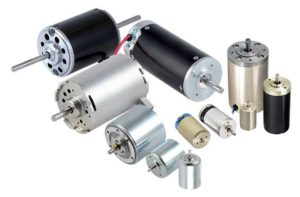
\includegraphics[width=.5\textwidth]{dc_motors}
\end{figure}

\column{0.5\textwidth}
{\small A DC motor is any of a class of rotary electrical motors that converts direct current electrical energy into mechanical energy.} 
{\scriptsize 
\begin{itemize}
    \item Simple.
    \item Low cost.
    \item High efficiency.
    \item No direction.
    \item Pair with reducer to achieve different behavior.
    \item Many applications: toys, ceiling fans, hydraulic pumps, electric cars/bikes, robots ...
\end{itemize}
}

\end{columns}
\hfill \\
A great explanation of \href{https://youtu.be/CWulQ1ZSE3c}{how does a DC motor works}.

\end{frame}

\begin{frame}
    \centering Let's have a race!
\end{frame}

\section{Raspberry Pi}
\begin{frame}{Introduction to Raspberry Pi}
        \begin{itemize}
            {\scriptsize
            \item The Raspberry Pi is a low cost, credit-card sized computer. It’s capable of doing everything you’d expect a desktop computer to do. 
            \item Raspberry Pi  has the ability to interact with the outside world, and has been used in a wide array of digital maker projects, from \href{https://youtu.be/_nBK8sAl9nw}{music machines} and \href{https://www.raspberrypi.org/blog/deter-package-thieves-from-your-porch-with-raspberry-pi/}{package thief alarm} to \href{https://projects.raspberrypi.org/en/projects/build-your-own-weather-station}{weather stations} and \href{https://projects.raspberrypi.org/en/projects/infrared-bird-box}{tweeting birdhouses}. 
            \item Of course, there are many Raspberry Pi powered \href{https://www.google.com/search?q=raspberry+pi+robots}{robots}
            }
        \end{itemize}
     
\end{frame}

\begin{frame}{Get Started}
        \begin{itemize}
            {\small
            \item \href{https://www.raspberrypi.org/software/}{Install} an operating system. 
            \item Set up a controllable LED. 
            }
        \end{itemize}
     
\end{frame}

 
\end{document}
